% !TEX program = pdflatex
% Cheat Sheet for Introduction to Communication System, Final Exam
\documentclass[UTF8,a4paper,10pt]{article}
\usepackage[UTF8,scheme=plain,linespread=.1]{ctex}
\usepackage[margin=.1in]{geometry}
\usepackage{multicol}
\setlength{\columnseprule}{1pt}
\usepackage{amsmath,amssymb,mathrsfs,bm}
\allowdisplaybreaks[4]
\providecommand{\abs}[1]{\left\lvert#1\right\rvert}
\providecommand{\norm}[1]{\left\lVert#1\right\rVert}
\providecommand{\re}{\,\mathrm{Re}\,}
\providecommand{\im}{\,\mathrm{Im}\,}
% \providecommand{\sgn}{\,\text{sgn}\,}
\providecommand{\sinc}{\,\mathrm{sinc}\,}
\providecommand{\rect}{\,\mathrm{rect}\,}
\usepackage{ulem}
\usepackage{calc}
\usepackage{tikz}
\usetikzlibrary{shapes.geometric, positioning, quotes, graphs}
\begin{document}
\scriptsize
\begin{multicols*}{2}
\noindent\textbf{通信系统架构}:\textbf{信源(source)输入}$\rightarrow$\textbf{采样(sampling)}(得时间离散幅值连续的模拟信号)$\rightarrow$\textbf{量化(quantization)}(得时间幅值均离散的数字信号)$\overset{\textbf{模拟序列}}{\longrightarrow}$\textbf{信源编码(source encoder)}(幅值转二进制;压缩,提高效率)$\overset{\textbf{二进制接口(binary interface)}}{\longrightarrow}$\textbf{信道编码(channel encoder)}(增加冗余,提高可靠性)$\rightarrow$\textbf{调制(modulation)}(转为模拟信号,因仅模拟信号可在物理世界传播;频分复用)$\rightarrow$\textbf{信道(channel)}(给定,不可控,概率性的;类型:有/无记忆,离散/连续)$\rightarrow$\textbf{解调(demodulation)}$\rightarrow$\textbf{信道解码(channel decoder)}(检错,纠错)$\rightarrow$\textbf{信源解码(source decoder)}(二进制序列解码)$\rightarrow$\textbf{查映射表(mapping table lookup)}(幅度离散转连续)$\rightarrow$\textbf{低通滤波(lowpass filter)}(恢复模拟信号)$\rightarrow$\textbf{输出(output)}\\
\textbf{信息论基础}\rule{\columnwidth-\widthof{信息论基础}}{.2pt}\\
\textbf{信息熵(information entropy)}:\textbf{离散rv}$X$所含信息量,$H(X)=-\sum_{x\in\mathcal{X}}p(x)\log_2p(x)$,其中$\mathcal{X}$-样本空间,$p(x)=P(X=x)$;事件越不确定,信息量越大;证:描述信息量须满足三条件,$H(\{p_i\})$关于$p_i$连续,$H(\{p_i=\frac{1}{n}\})$关于$n$单增,$H(\{p_i\})$可分解,$H(p_1,p_2,p_3)=H(p_1)+(1-p_1)H(\frac{p_2}{1-p_1},\frac{p_3}{1-p_1})$,故$H$必有形式$H(X)=-K\sum p(x)\log_2p(x)$;$H(X)=E[-\log_2p(x)]$;$H(X)\geq 0$,若$X$确定,$H(X)=0$;$H(X)\leq\log_2\abs{\mathcal{X}}$,若无约束条件,均匀分布下$H(X)$最大\\
\textbf{联合熵(joint entropy)}:$X$,$Y$共同所含信息量,$H(X,Y)=-\sum_{x\in\mathcal{X},y\in\mathcal{Y}}p(x,y)\log_2p(x,y)$;若$X$,$Y$独立,$H(X,Y)=H(X)+H(Y)$;证:$H(X,Y)=-\sum_{x,y}p(x,y)\log_2p(x,y)=-\sum_{x,y}p(x)p(y)\log_2p(x)p(y)=-\sum_{x,y}p(x)p(y)\log_2p(x)-\sum_{x,y}p(x)p(y)\log_2p(y)=-\sum_xp(x)\log_2p(x)-\sum_yp(y)\log_2p(y)=H(X)+H(Y)$\\
\textbf{条件熵(conditional entropy)}:已知$Y$所含信息时,$X$所剩信息,$H(X\vert Y)=-\sum_{x\in\mathcal{X},y\in\mathcal{Y}}p(x,y)\log_2p(x\vert y)$;$H(X,Y)=H(X)+H(Y\vert X)$;证:$H(X,Y)=-\sum_{x,y}p(x,y)\log_2p(x,y)=-\sum_{x,y}p(x,y)\log_2p(x)p(y\vert x)=-\sum_xp(x)\log_2p(x)-\sum_{x,y}p(x,y)\log_2p(y\vert x)=H(X)+H(Y\vert X)$;$H(X\vert Y)=\sum_yp(y)H(X\vert Y=y)$;$X(X)\geq H(X\vert Y)$\\
\textbf{互信息(mutual info)}:$X$,$Y$的互相关性,$I(X;Y)=\sum_{x\in\mathcal{X},y\in\mathcal{Y}}p(x,y)\log_2\frac{p(x,y)}{p(x)p(y)}$;作用类似皮尔森相关系数,但范围不局限于$[-1,1]$,而是$[0,\infty)$,计算角皮尔森相关系数复杂;另一物理意义:已知$Y$导致$X$不确定性减少量,$H(X;Y)=H(Y;X)=H(X)-H(X\vert Y)=H(Y)-H(Y\vert X)=H(X)+H(Y)-H(X,Y)$;另一物理意义:联合分布与单边分布差距,$I(X;Y)=D(p(x,y)\Vert p(x)p(y))$,其中KL散度$D(p(x)\Vert q(x))=\sum_x\log_2\frac{p(x)}{q(x)}$;$I(X;X)=H(X)$;$I(X;\text{const})=0$\\
\textbf{微分熵(differential entropy)}:\textbf{连续rv}$X$所含信息量,$h(X)=-\int_{-\infty}^{+\infty}f(x)\log_2f(x)\,\mathrm{d}x$,其中$f(x)$-$X$的PDF;$h(X)=E(-\log_2f(x))$;$f\in(-\infty,+\infty)$;对$X\in u(a,b)$,$h(X)=-\log_2(b-a)$;给定方差下,高斯分布的微分熵最大,对$X\sim N(0,\sigma^2)$,$f(x)=\frac{1}{\sqrt{2\pi\sigma^2}}e^{-\frac{x^2}{2\sigma^2}}$,$h(X)=\int_{-\infty}^{+\infty}f(x)[\frac{x^2}{2\sigma^2}+\ln\sqrt{2\pi\sigma^2}]=\frac{E[X^2]}{2\sigma^2}+\frac{1}{2}\ln 2\pi\sigma^2=\frac{1}{2}+\frac{1}{2}\ln 2\pi\sigma^2(\text{nats})=\frac{1}{2}\log_22\pi e\sigma^2(\text{bits})$\\
\textbf{连续rv$X$,$Y$的互信息}:$I(X;Y)=\iint_{-\infty}^{+\infty}f(x,y)\log_2\frac{f(x,y)}{f(x)f(y)}\,\mathrm{d}x\,\mathrm{d}y$;$I(X;Y)=h(X)-h(X\vert Y)$\\
\textbf{信源编码}\rule{\columnwidth-\widthof{信源编码}}{.2pt}\\
以下讨论针对\textbf{离散无记忆信源(discrete memoryless sources, DMS)}:由字符表(alphabet)$\mathcal{X}$中按一定概率随机选择字符输出为无穷序列$X_1,\cdots$,$X_i$i.i.d$\forall i$;\textbf{平均码长}:$\bar{L}=\sum_xp(x)l(x)$\\
\textbf{定长码(fixed-length code)}:每个字符所需码长$\log_2M\leq L=\lceil\log_2M\rceil\leq\log_2M+1$,编码效率低,但分词快,收到即解码;视$n$个字符为一整体用定长码编码,$L=\lceil\log_2M^n\rceil$,平均码长$\log_2M\leq\bar{L}=\frac{1}{n}\lceil\log_2M^n\rceil\leq\log_2M+\frac{1}{n}$\\
\textbf{可变长码}:不同字符对应码长不一定相等;\textbf{非奇异(non-singular)码}:字符与编码一一对应,否则为\textbf{奇异(singular)码};\textbf{唯一可解(unique decodable)码}:可分词;\textbf{瞬时(instantaneous)码}:收到即解码\\
\textbf{无前缀(prefix-free)码}:任一字符编码非其余任一字符编码的前缀,各字符编码均在二叉树叶上,是一种可变长瞬时码;当为\textbf{霍夫曼树}(出叶外任一节点要么有$0$个要么有$2$个子节点),编码最优\\
\textbf{Kraft定理}:$\sum_{x\in\mathcal{X}}e^{-l(x)}\leq 1$,取等时编码效率最高\\
\textbf{最优平均码长范围}:$\bar{L}_{\min}=\sum_{l_1,\cdots,l_M}\sum_ip_il_i$s.t.$\sum_i2^{-l_i}\leq 1$,$\frac{\partial[\bar{L}_{\min}+\lambda\sum_i(2^{-l_i}-1)]}{\partial}=0\Rightarrow p_i-\lambda(\ln 2)2^{-l_i}=0$,为编码效率最高,$\sum_i2^{-l_i}=1$,取$\lambda=\frac{1}{\ln 2}\Rightarrow l_i=-\log_2p_i$,对$p_i=\frac{1}{2^n}\forall i$,$\bar{L}_{\min}=H(X)$,一般地,$H(X)\leq\bar{L}_{\min}<H(X)+1$\\
\textbf{霍夫曼(Huffman)编码}:将所有字符按出现概率排列,出现概率最小的两个字符作为子节点,以其父节点(对应出现概率为两个子节点之和)为新的子节点,与剩下出现概率最小的字符作为子节点,循环至二叉树包括所有字符;从一数组按一定概率抽出一个数,如何用判断题最快地问出该数:将这组数按概率霍夫曼编码,从最低位往高位问\\
\textbf{香农第一定理(Shannon's 1st thm)}:$X$为熵为$H(X)$的DMS,对任何码率(平均码长)$R>H(X)$,存在无损信源编码方式,对$R<H(X)$,不存在无损信源编码方式\\
\textbf{采样}\rule{\columnwidth-\widthof{采样}}{.2pt}\\
$x(t)$的采样信号:$x_{\delta}(t)=\sum_{k=-\infty}^{+\infty}x(kT)\delta(t-kT)$,其中$T$-采样周期,采样频率$f_s=\frac{1}{T}$\\
\textbf{采样定理(sampling thm)}:带限为$W$的平稳随机过程$X(t)=\sum_{k=-\infty}^{+\infty}X(\frac{k}{2W})\sinc(2Wt-k)$,其中采样周期$T=\frac{1}{2W}$,采样频率$f_s=2W$;%
    证:$[-W,W]$频率范围内$x_{\delta}(t)$离散时间傅里叶变换$\hat{x}(f)=\sum_kx_ke^{-2\pi jkf/2W}\Pi(\frac{f}{2W})=\sum_kx_k\hat{\phi}_k(f)$,其中$x_k=\frac{1}{2W}\int_{-W}^W\hat{x}(f)e^{2\pi jkf/2W}\,\mathrm{d}f$,$\hat{\phi}_k(f)=e^{-2\pi jkf/2W}\Pi(\frac{f}{2W})\Rightarrow\phi_k(t)=2W\sinc(2Wt-k)\Rightarrow x(t)=\sum_kx_k\phi_k(t)=\sum_k2Wx_k\sinc(2Wt-k)$,$\because\sinc(k)=\delta_{k0}$,$\therefore x(\frac{k}{2W})=2Wx_k\Rightarrow x(t)=\sum_kx(\frac{k}{2W})\sinc(2Wt-k)$\\
\textbf{混叠}:信号$x(t)$采样估计$s(t)=\sum_{k=-\infty}^{+\infty}x(kT)\sinc(Tt-k)$的频谱$\hat{s}(f)=\sum_{m=-\infty}^{+\infty}\hat{x}(f+\frac{m}{T})\Pi(fT)$;%
    频域:$\hat{x}(f)=\lim_m\hat{v}_m(f)$,其中第$m$段$\hat{v}_m(f)=\hat{x}(f)\Pi(\frac{f}{2W}-m)\Rightarrow v_m(t)=\sum_kv_m(kT)\sinc(\frac{t}{T}-k)e^{2\pi jmt/T}=\sum_kv_m(kT)\psi_{m,k}(t)\Rightarrow x(t)=\sum_{m,k}v_m(kT)\sinc(\frac{t}{T}-k)e^{2\pi jmt/T}$,若$x(t)$带限$W$,仅$m=0$项$\neq 0$,$s(t)=x(t)$,否则$s(t)=\sum_{k,m}v_m(kT)\sinc(\frac{t}{T}-k)\neq x(t)$;%
    时域:$x(t)=\sum_mv_m(t)$,$s(t)=\sum_{k,m}v_m(kT)\sinc(\frac{t}{T}-k)=\sum_ms_m(t)$,其中$v(t)=\sum_kv_m(kT)\sinc(\frac{t}{T}-k)e^{2\pi jmt/T}$,$s_m(t)=\sum_kv_m(kT)\sin(\frac{t}{T}-k)=v_m(t)e^{-2\pi jmt/T}\Rightarrow\hat{s}_m(f)=\hat{v}(f+\frac{m}{T})=\hat{x}(f+\frac{m}{T})\Pi(fT)\Rightarrow\hat{s}(f)=\sum_m\hat{x}(f+\frac{m}{T})\Pi(fT)$\\
\textbf{量化}\rule{\columnwidth-\widthof{量化}}{.2pt}\\
连续幅值$U_1,\cdot$转离散$V_1,\cdots$;%
    \textbf{标量量化}:$1$个采样映射$1$个数,$U=u\in\mathcal{R}_j=(b_{j-1},b_j)\rightarrow V=a_j$;%
    \textbf{均方差(mean square error,MSE)}:$E[\abs{U-V}^2]$;%
    目标:给定pdf$f_U(u)$,选\textbf{量化区间(quantization intervals)}$\{\mathcal{R}_j\}$\&\textbf{代表点(representation points)}$\{a_j\}$以最小化MSE;%
    目前无系统性最优方法,故分解为$2$个小目标:\textcircled{1}给定$\{a_j\}$,选$\{\mathcal{R}_j\}$,MSE$=\sum_{j=1}^M\int_{b_{j-1}}^{b_j}f_U(u)(u-a_j)^2\,\mathrm{d}u$,$\frac{\partial\text{MSE}}{\partial b_j}=f_U(b_j)(b_j-a_j)^2-f_U(b_j)(b_j-a_{j-1})^2=0\Rightarrow b_j=\frac{a_j+a_{j-1}}{2}$;%
    \textcircled{2}:给定$\{\mathcal{R}_j\}$,选$\{a_j\}$,$\frac{\partial\text{MSE}}{\partial a_j}=-2\int_{\mathcal{R}_j}f_U(u)u\,\mathrm{d}u+2\int_{\mathcal{R}_j}f_U(u)a_j\,\mathrm{d}u=0\Rightarrow a_j=\frac{\int_{\mathcal{R}_j}uf_U(u)\,\mathrm{d}u}{\int_{\mathcal{R}_j}f_U(u)\,\mathrm{d}u}=E[U\vert\mathcal{R}_j]$;%
    此即最优量化的必要条件;%
    \textbf{Lloyd-Max算法}:初始化$a_1,\cdots,a_M\rightarrow$\textcircled{1}$\rightarrow$\textcircled{2}$\rightarrow$迭代足次;%
    \textbf{向量量化}:相邻多个采样映射多个数;%
    \textcircled{1}:取$\{(a_j,a_{j'})\}$邻近两点中垂线以划分$\{\mathcal{R}_j\}$;%
    \textcircled{2}:$(a_j,a_{j'})=E[(U_1,U_2)\vert\mathcal{R}_j]$\\
\textbf{定熵量化}:为便于信源编码,在给定熵(即信源编码的平均码长)$H(V)=\bar{L}$下量化;%
    若高精度(high-rate)量化,则等间距量化;%
    证:拉格朗日函数$L=E[(U-V)^2]+\lambda H(V)$,若$f_U(u)=f_1(\text{长}L_1\text{的区间}1),f_2(\text{长}L_2\text{的区间}2)$,则先将两区间等间距分为$M_i=\frac{L_i}{\Delta_i}$份,代表点$\{a_j^{(i)}\}$,$E[(U-V)^2]=\sum_{i=1,2}\sum_{j=1}^{M_i}\int_{a_j^{(i)}-\Delta_i/2}^{a_j^{(i)}+\Delta_i/2}f_i(u-a_j^{(i)})^2\,\mathrm{d}u=\frac{f_1L_1\Delta_1^2}{12}+\frac{f_2L_2\Delta_2^2}{12}$,$H(V)=-\sum_{i=1,2}M_if_i\Delta_i\log_2 f_i\Delta_i=-f_1L_1\log_2(f_1\Delta_1)-f_2L_2\log_2(f_2\Delta_2)$,拉格朗日乘子法$\frac{\partial L}{\partial\Delta_i}=\frac{\Delta_if_iL_i}{6}-\frac{\lambda f_iL_i}{\Delta_i}=0\forall i\Rightarrow\Delta_1^2=\Delta_2^2=6\lambda$,推广即得,若pdf足够平缓,则等间距量化近似最优;%
    此时MSE$\approx\frac{\Delta^2}{12}$,$H(V)\approx h(U)-\log_2\Delta\Rightarrow$MSE$\approx\frac{2^{2h(U)-2\bar{L}}}{12}$;%
    若$\Delta\rightarrow\frac{\Delta}{2}$,MSE$\rightarrow\frac{1}{4}$MSE,$\bar{L}\rightarrow\bar{L}+1$;%
    工程中$f(u)$定义域或$(-\infty,+\infty)$,则仅处理主要概率分布的区间\\
\textbf{向量空间和信号空间(vector spaces \& signal space)}\rule{\columnwidth-\widthof{向量空间和信号空间(vector spaces \& signal space)}}{.2pt}\\
$n$维\textbf{向量(vector)}:$\bm{v}=(v_1,\cdots,v_n)^T$;%
    \textbf{向量空间}$\mathcal{V}$:一组向量$\bm{v}$的集合,操作此组向量的规则及一组标量$\alpha\in\mathbb{F}$(可实可复);%
    性质:$\bm{u}+\bm{v}=\bm{v}+\bm{u}$,%
    $\forall\alpha$,$\beta$,$\alpha(\beta\bm{v})=(\alpha\beta)\bm{v}$,%
    $\alpha(\bm{u}+\bm{v})=\alpha\bm{u}+\alpha\bm{v}$,%
    $(\alpha+\beta)\bm{v}=\alpha\bm{v}+\beta\bm{v}$,%
    $\norm{v}=\sqrt{\sum_{i=1}^n\abs{v_i}^2}$\\
\textbf{内积(inner product)}:$\langle\bm{v}_1,\bm{v}_2\rangle=\bm{v}_1\cdot\bm{v}_2=\sum_{i=1}^nv_{1i}v_{2i}^*=\bm{v}_2^{\dagger}\bm{v}_1$,其中$\bm{v}_1=(v_{11},\cdots,v_{1n})^T$,$\bm{v}_2=(v_{21},\cdots,v_{2n})^T$;%
    性质:$\langle\bm{v}_1,\bm{v}_2\rangle=\langle\bm{v}_2,\bm{v}_1\rangle^*$,%
    $\langle\bm{v}_1,\bm{v}_2\rangle+\langle\bm{v}_2,\bm{v}_1\rangle=2\re[\langle\bm{v}_1,\bm{v}_2\rangle]$,%
    $\bm{v}_1$\&$\bm{v}_2$\textbf{正交}$\Leftrightarrow\langle\bm{v}_1,\bm{v}_2\rangle=0$,%
    $\{\bm{v}_k\}$正交$\Leftrightarrow\langle\bm{v}_i,\bm{v}_j\rangle=0\forall i\neq j$,%
    $\{\bm{v}_k\}$\textbf{正交归一}$\Leftrightarrow\{\bm{v}_k\}$正交且$\norm{\bm{v}_i}=1\forall i$\\
$\cos(\angle(\bm{v},\bm{u}))=\frac{\langle\bm{v},\bm{u}\rangle}{\norm{\bm{v}}\norm{\bm{u}}}$;%
    与$\bm{u}$同向的单位向量:$\frac{\bm{u}}{\norm{\bm{u}}}$;%
    $\bm{v}$在$\bm{u}$上\textbf{投影(projection)}:$\bm{v}_{\bm{u}}=\frac{\langle\bm{v},\bm{u}\rangle}{\norm{\bm{u}}^2}\bm{u}$,$\bm{v}\perp\bm{u}$分量:$\bm{v}_{\perp\bm{u}}=\bm{v}-\bm{v}_{\vert\bm{u}}$;%
    \textbf{施瓦茨不等式}:$\abs{\langle\bm{u},\bm{v}\rangle}\leq\norm{\bm{u}}\norm{\bm{v}}$,当且仅当$\bm{v}_1=a\bm{v}_2$或$\bm{v}_2=a\bm{v}_1$时取等;%
    证:$\cos(\angle(\bm{v},\bm{u}))=\frac{\langle\bm{v},\bm{u}\rangle}{\norm{\bm{v}}\norm{\bm{u}}}\leq 1$;%
    \textbf{三角不等式}:$\norm{\bm{v}_1+\bm{v}_2}\leq\norm{\bm{v}_1}+\norm{\bm{v}_2}$;
    若$\bm{v}_1$\&$\bm{v}_2$正交,$\norm{\bm{v}_1+\bm{v}_2}^2=\norm{\bm{v}_1}^2+\norm{\bm{v}_2}^2$\\
\textbf{线性不独立}:若$\sum_{j=1}^n\alpha_j\bm{v}_j=0$,其中$\exists\alpha_i\neq 0$;%
    否则\textbf{线性独立};%
    若$\forall\bm{v}$可表为$\bm{v}_1,\cdots,\bm{v}_n$的线性组合,则$\bm{v}_1,\cdots,\bm{v}_n$张成$\mathcal{V}$;%
    若$\bm{v}_1,\cdots,\bm{v}_n$张成$\mathcal{V}$且线性独立,则$\bm{v}_1,\cdots,\bm{v}_n$为$\mathcal{V}$的一组\textbf{基};%
    若$\bm{v}_1,\cdots,\bm{v}_m$张成$\mathcal{V}$且线性不独立,其中$\mathcal{V}$-一非平庸有限维向量空间,其一子集$\bm{v}_1,\cdots,\bm{v}_n$为$\mathcal{V}$的基;%
    若$\bm{v}_1,\cdots,\bm{v}_m$线性独立而无法张成$\mathcal{V}$,存在$\mathcal{V}$的一组基包含$\bm{v}_1,\cdots,\bm{v}_n$;%
    $\mathcal{V}$的每组基均包含相等数量的基矢\\
$\bm{v}$在$\mathcal{S}$上\textbf{投影}:$\bm{v}_{\vert\mathcal{S}}=\sum_{j=1}^n\langle\bm{v},\bm{\phi}_j\rangle\bm{\phi}_j$,其中$\bm{\phi}_1,\cdots,\bm{\phi}_n$-$\mathcal{S}$的一组正交归一基\\
\textbf{格拉姆-施密特正交化}:给定$\mathcal{V}$的任一组基$\{\bm{s}_1,\cdots,\bm{s}_n\}$,得一组正交归一基$\{\bm{\phi}_1,\cdots,\bm{\phi}_n\}$,\textcircled{1}$\bm{\phi}_1=\frac{\bm{s}_1}{\norm{\bm{s}_1}}$,\textcircled{2}$(\bm{s}_{k+1})_{\perp\mathcal{S}_k}=\bm{s}_{k+1}-(\bm{s}_{k+1})_{\vert\mathcal{S}_k}=\bm{s}_{k+1}-\sum_{j=1}^k\langle\bm{s}_{k+1},\bm{\phi}_j\rangle\bm{\phi}_j$,其中$\mathcal{S}_k$-$\{\bm{\phi}_1,\cdots,\bm{\phi}_k\}$张成的子空间,\textcircled{3}$\bm{\phi}_{k+1}=\frac{(\bm{s}_{k+1})_{\perp\mathcal{S}_k}}{\norm{(\bm{s}_{k+1})_{\perp\mathcal{S}_k}}}\forall k=1,\cdots,n-1$\\
信号$x(t)$的\textbf{能量(范数)}:$E=\norm{x(t)}^2=\int_{-\infty}^{+\infty}\abs{x(t)}^2\,\mathrm{d}t$;%
    \textbf{内积}:$\langle x_1(t),x_2(t)\rangle=\int_{-\infty}^{+\infty}x_1(t)x_2^*(t)\,\mathrm{d}t$;%
    $x_1(t)$\&$x_2(t)$\textbf{正交}$\Leftrightarrow\langle x_1(t),x_2(t)\rangle=0$;%
    \textbf{正交归一}$\Leftrightarrow$正交且$E=1$;%
    \textbf{线性无关}:任意信号无法表为其余信号线性组合;%
    \textbf{三角不等式}:$\norm{x_1(t)+x_2(t)}\leq\norm{x_1(t)}+\norm{x_2(t)}$;%
    \textbf{施瓦茨不等式}:$\abs{\langle x_1(t),x_2(t)\rangle}\leq\norm{x_1(t)}\norm{x_2(t)}$\\
\textbf{格拉姆-施密特正交化}:给定$\{s_m(t)\}_{m=1}^M$,得一组正价归一信号$\{\phi_1(t),\cdots,\phi_M(t)\}$,\textcircled{1}$\phi_1(t)=\frac{s_1(t)}{\sqrt{E_1}}$,\textcircled{2}$\gamma_{k+1}(t)=s_{k+1}(t)-\sum_{i=1}^k\langle s_{k+1},\phi_i(t)\rangle\phi_i(t)$,\textcircled{3}$\phi_{k+1}(t)=\frac{\gamma_{k+1}(t)}{\sqrt{E_{k+1}}}\forall k=1,\cdots,M-1$\\
\textbf{在$\mathcal{L}_2$上正交归一展开}:用$u(t)=\sum_{m=1}^n\alpha_m\phi_m(t)=(\alpha_1,\cdots,\alpha_n)^T$近似$v(t)$,其中$\{\phi_m(t)\}_{m=1}^n$正交归一,为最小化误差$e(t)=v(t)-u(t)$的能量,$\alpha_m=\langle v(t),\phi_m(t)\rangle$从而$\langle e(t),\phi_m(t)\rangle=\int_{-\infty}^{+\infty}e(t)\phi_m^*(t)\,\mathrm{d}t=0$\\
\textbf{带通信号}:$x(t)=\re[u(t)e^{j2\pi f_0t}]=\sum_{m=1}^n\re[u_m]\re[\phi_m(t)e^{j2\pi f_0t}]-\sum_{m=1}^n\im[u_m]\im[\phi_m(t)e^{j2\pi f_0t}]=\sum_{m=1}^n[\frac{\re[u_m]}{\sqrt{2}}\psi_m(t)+\frac{\im[u_m]}{\sqrt{2}}\tilde{\psi}_m(t)]$,$\bm{x}=(\frac{\re[u_1]}{\sqrt{2}},\frac{\im[u_1]}{\sqrt{2}},\cdots,\frac{\re[u_n]}{\sqrt{2}},\frac{\im[u_n]}{\sqrt{2}})^T$,其中原基带信号$u(t)=\sum_{m=1}^nu_m\phi_m(t)$,$\bm{u}=(u_1,\cdots,u_n)^T$,$\{\phi_m(t)\}_{m=1}^n$-$u(t)$的一组正交归一基,$u_m=\langle u(t),\phi_m(t)\rangle$,\textbf{带通信号的正交归一基}$\{\psi_m(t)=\sqrt{2}\re[\phi_m(t)e^{j2\pi f_0t}],\tilde{\psi}_m(t)=-\sqrt{2}\im[\phi_m(t)e^{j2\pi f_0t}]\}$;
    若$u(t)=A\sqrt{E}\phi(t)$,其中$\norm{\phi(t)}=1$且$\phi(t)\in\mathbb{R}$,$\bm{x}=(\frac{\re[A]\sqrt{E}}{\sqrt{2}},\frac{\im[A]\sqrt{E}}{\sqrt{2}})^T$,\textbf{带通信号的正交归一基}$\{\sqrt{2}\re[\phi(t)e^{j2\pi f_0t}]=\sqrt{2}\phi(t)\cos(2\pi f_0t),\sqrt{2}\im[\phi(t)e^{j2\pi f_0t}]=\sqrt{2}\phi(t)\sin(2\pi f_0t)\}$\\
\textbf{调制\&解调}\rule{\columnwidth-\widthof{调制\&解调}}{.2pt}\\
二进制输入$\overset{\{0,1\}^n}{\rightarrow}$编码(encoder)$\overset{\{u_k\in\mathcal{A}\}}{\rightarrow}$基带调制(baseband modulation,$p(t)$)\\
    $\overset{u(t)=\sum_ku_kp(t-kT)}{\rightarrow}$载频(base2passband)$\overset{x(t)=2\re[u(t)e^{j2\pi f_ct}]}{\rightarrow}$信道$\overset{y(t)=x(t)+\text{WGN}}{\rightarrow}$\\
    去载频(pass2baseband)$\rightarrow$匹配滤波器(matched filter,$q(t)$)$\rightarrow$采样$\overset{\{v_k\}^n}{\rightarrow}$检测(detection)\\
    $\overset{\{\tilde{u}_k\}^n}{\rightarrow}$星座图反映射(constellation inverse mapping)$\overset{\{0,1\}^n}{\rightarrow}$二进制输出\\
\textbf{脉冲调幅(pulse amplitude modulation,PAM)}:${0,1}^n\rightarrow\{u_k\in\mathbb{R}\}$,$u(t)=\sum_ku_k(t)=\sum_ku_kp(t-kT)$,其中$\{p(t-kT)\}$正交,$x(t)=2\re[u(t)e^{j2\pi f_ct}]$;%
    \textbf{2-PAM}:$0\rightarrow u_k=+1$,$1\rightarrow u_k=-1$;%
    \textbf{4-PAM}:$00\rightarrow u_k=-3$,$01\rightarrow-1$,$10\rightarrow+1$,$11\rightarrow+3$;%
    \textbf{M-PAM}:$b$bit(s)$\rightarrow$星座图$\mathcal{A}=\{a_1,\cdots,a_M\}$,其中$a_j\in\mathbb{R}$,$M=2^b$,\textbf{位间隔(bit interval)}:传输单比特平均耗时$T_b$,\textbf{信号间隔(signal interval)}:单个符号平均耗时$T=T_b\times b$,\textbf{比特率(bit rate)}:单位时间平均传输信号位数$R_b=\frac{1}{T_b}$,\textbf{码率(signal/symbol rate)}:单位时间平均传输符号数$R_s=\frac{1}{T}=\frac{R_b}{b}$,设$U_1,\cdots$iid$\sim P(U_k=a_m)=p_m$,其中$k$-时间序号,星座图序号$m\in\{1,\cdots,M\}$,单个符号$a_m$能耗:$E_m=\int\abs{a_mp(t)}^2\,\mathrm{d}t=a_m^2E_p$,单符号平均能耗:$E_{\text{avg}}=\sum_{m=1}^Mp_mE_m$,单比特平均能耗:$E_{b,\text{avg}}=\frac{E_{\text{avg}}}{b}$,平均功率:$P_{\text{avg}}=\frac{E_{\text{avg}}}{T}=\frac{E_{b,\text{avg}}}{T_b}$;%
    星座图$\mathcal{A}=\{-\frac{d(M-1)}{2},\cdots,-\frac{d}{2},\frac{d}{2},\cdots,\frac{d(M-1)}{2}\}$,通常$P_m=\frac{1}{M}$,则$E_{\text{avg}}=\frac{2}{M}(\frac{d}{2})^2[1^2+3^2+\cdots+(M-1)^2]=\frac{d^2(M^2-1)E_p}{12}$,$b$越大,抗噪性能越好,误码率越低,但功耗越高;%
    若噪声$<\frac{d}{2}$,可正确检测\\
\textbf{相位偏移调制(phase-shift keying,PSK)}:星座图中符号等模,相位不同;%
    \textbf{B(inary)PSK}$=$2-PAM:$0\rightarrow u_k=1$,$1\rightarrow e^{j\pi}$;%
    \textbf{QPSK}:$00\rightarrow u_k=1$,$01\rightarrow e^{j\pi/2}$,$10\rightarrow e^{j\pi}$,$11\rightarrow e^{j3\pi/2}$;%
    \textbf{BF(req)SK}:$0\rightarrow u_k(t)=A\cos(2\pi\Delta ft)$,$1\rightarrow A\cos(4\pi\Delta ft)$;%
    阶数越大,抗噪声性能越好,码率(传输效率)越高\\
\textbf{正交调幅(quadrature amplitude modulation,QAM)}:星座图中符号可为任意复数,$x(t)=2\re[u(t)]\cos(2\pi f_ct)-2\im[u(t)]\sin(2\pi f_ct)=u(t)e^{j2\pi f_ct}+u^*(t)e^{-j2\pi f_ct}$;%
    实现方法1:当基带信号$u(t)$带宽$B_b<f_c$,$\hat{u}(f-f_c)$与$\hat{u}(f+f_c)$无重叠,发送端$x^+(t)=u(t)e^{j2\pi f_ct}$,$x(t)=x^+(t)+[x^+(t)]^*$,接收端用希尔伯特滤波器$\hat{h}(f)=1(h>0)$,$0(f\leq 0)$恢复$x^+(t)$,去载波得$u(t)$;%
    实现方法2如图,匹配滤波器得$r(t)=\int u(\tau)q(t-\tau)\,\mathrm{d}\tau=\int\sum_ku_kp(\tau-kT)q(t-\tau)\,\mathrm{d}\tau=\sum_ku_kg(t-kT)$,其中$g(t)=p(t)*q(t)$,需满足$r(jT)=u_j$,则$g(t)$需为理想Nyquist,$g(kT)=\delta_{k0}\Leftrightarrow\sum_k\hat{g}(f+\frac{k}{T})\Pi(fT)=T\Pi(fT)$(奈奎斯特准则(Nyquist criterion),$\hat{g}(f)$关于$(W_b=\frac{1}{2T},\frac{T}{2})$对称(bandedge symmetry)),否则有符号间干扰(intersymbol interference,ISI),不存在$g$带宽$B_b<W_b$,若$B_b=W_b$,则必$g(t)=\sinc\frac{t}{T}$,若$W_b\leq B_b\leq 2W_b$,则$g(t)$有多种选择,给定$g(t)$后选$\hat{p}(f)=\hat{q}^*(f)$,则$\abs{\hat{p}(f)}=\abs{\hat{q}(f)}=\sqrt{\hat{g}(f)}$带宽相等,$q(t)=p^*(-t)$,$g(t)=\int p(\tau)q(t-\tau)\,\mathrm{d}\tau=\int p(\tau)p^*(\tau-t)\,\mathrm{d}\tau$,$g(kT)=\int p(\tau)p^*(\tau-kT)\,\mathrm{d}\tau=\int p(\tau-jT)p^*(\tau-(k+j)T)\,\mathrm{d}\tau$,$\because g(t)$理想Nyquist,$\{p(t-kT)\}$正交归一,以$T$为周期采样得$u_k=\langle u(t),p(t-kT)\rangle$\\
\textbf{自由度(degree of freedom,DoF)}:单位时间传输符号数,$B_b$-基带带宽,$W=2B_b$-带通带宽,$T$-信号间隔(符号周期),$T_0$-总传输时长,PAM每$T$发送$1$个实符号,$T_0$发送$\frac{T_0}{T}$,real DoF$=1$,QAM每$T$发送$1$个复符号,complex DoF$=1$,real DoF$=2$,在Nyquist准则$B_b\geq\frac{1}{2T}$下$B_b$应尽可能小,工程上通常$B_b\approx(1.05\sim 1.10)\frac{1}{2T}$,PAM$T_0$内发送$\frac{T_0}{T}\approx 2T_0B_b$个实符号,QAM$T_0$内发送$\frac{T_0}{T}\approx 2T_0B_b$个复符号$=4T_0B_b$个实符号\\
应对多径效应,需引入符号间隔或均衡器(equalizer)$C(t)$于接收器采样之后,需满足$Z$变换$C(z)=\frac{1}{G(z)}$或$E[e_kv_{k-j}^*]=0\forall j$,其中$e_k=u_k-\hat{u}_k$,$\hat{u}_k=\sum_{j=-K}^Kc_jv_{k-j}$\\
\textbf{检测}\rule{\columnwidth-\widthof{检测}}{.2pt}\\
发送$U\in\mathcal{A}$,接收$V$,检测得$\tilde{U}\in\mathcal{A}$,\textbf{先验概率(prior probability)}:发送$a_j$的概率,$p_U(a_j)$,通常建模为均匀分布,\textbf{后验(posterior)概率}:接收$v$的前提下发送$a_j$的概率,$p_{U\vert V}(a_j\vert v)$,\textbf{似然(likelihood)概率}:发送$a_j$的前提下接收$v$的概率,$f_{V\vert U}(v\vert a_j)$,通常建模为正态分布\\
\textbf{最大后验概率(maximum posterior proba,MAP)估计}:$\tilde{U}=\arg\max_{a_j}[p_{U\vert V}(a_j\vert v)]$;%
    若$U=\left\{\begin{array}{ll}
        0\rightarrow a_0,&p_0\\
        1\rightarrow a_1,&p_1
    \end{array}\right.$,$p_{U\vert V}(a_0\vert v)\underset{\tilde{U}=1}{\overset{\tilde{U}=0}{\gtreqless}}p_{U\vert V}(a_1\vert v)\Rightarrow\frac{p_0f_{V\vert U}(v\vert 0)}{f_V(v)}\underset{\tilde{U}=1}{\overset{\tilde{U}=0}{\gtreqless}}\frac{p_1f_{V\vert U}(v\vert 1)}{f_V(v)}\Rightarrow$似然比(likelihood ratio)$\Lambda(v)=\frac{f_{V\vert U}(v\vert 0)}{f_{V\vert U}(v\vert 1)}\underset{\tilde{U}=1}{\overset{\tilde{U}=0}{\gtreqless}}\frac{p_1}{p_0}=\eta$;%
    \textbf{误码率}:Pr$(e)=p_0\mathrm{Pr}(e\vert U=0)+p_1\mathrm{Pr}(e\vert U=1)$,其中Pr$(e\vert U=0)=\mathrm{Pr}(\Lambda(V)<\eta\vert U=0)=\int_{\mathcal{R}_1}f_{V\vert U}(v\vert 0)\,\mathrm{d}v$,Pr$(e\vert U=1)=\mathrm{Pr}(\Lambda(V)\geq\eta\vert U=1)=\int_{\mathcal{R}_0}f_{V\vert U}(v\vert 1)\,\mathrm{d}v$,$\mathcal{R}_0=\{v:\Lambda(v)\geq\eta\}$,$\mathcal{R}_1=\{v:\Lambda(v)<\eta\}$;%
    \textbf{白高斯噪声(WGN)下2PAM}:$U=\left\{\begin{array}{l}
        0\rightarrow a\\
        1\rightarrow -a
    \end{array}\right.$,$V=U+Z$,其中噪声$Z\sim\mathcal{N}(0,N_0/2)$,$f_{V\vert U}(v\vert 0)=\frac{1}{\sqrt{\pi N_0}}e^{-\frac{(v-a)^2}{N_0}}$,$f_{V\vert U}(v\vert 1)=\frac{1}{\sqrt{\pi N_0}}e^{-\frac{(v+a)^2}{N_0}}$,MAP准则:$\Lambda(v)=e^{\frac{4av}{N_0}}\underset{\tilde{U}=1}{\overset{\tilde{U}=0}{\gtreqless}}\eta\Rightarrow$对数似然比(logarithm likelihood ratio)LLR$(v)=\ln[\Lambda(v)]=\frac{4av}{N_0}\underset{\tilde{U}=1}{\overset{\tilde{U}=0}{\gtreqless}}\ln\eta\Rightarrow v\underset{\tilde{U}=1}{\overset{\tilde{U}=0}{\gtreqless}}\frac{N_0\ln\eta}{4a}$,误码率Pr$(e\vert U=1)=Q(\frac{a+(N_0/4a)\ln\eta}{\sqrt{N_0/2}})=Q(\frac{a}{\sqrt{N_0/2}}+\frac{\sqrt{N_0/2}}{2a}\ln\eta)$,Pr$(e\vert U=0)=Q(\frac{a-(N_0/4)\ln\eta}{\sqrt{N_0/2}})=Q(\frac{a}{\sqrt{N_0/2}}+\frac{\sqrt{N_0/2}}{2a}\ln\eta)$,若$\eta=1$,Pr$(e\vert U=1)=\mathrm{U}(e\vert U=0)=Q(\frac{a}{\sqrt{N_0/2}})=Q(\sqrt{\frac{2E_b}{N_0}})$,其中每比特能耗$E_b=a^2$;%
    \textbf{非对等(non-antipodal)信号}:$U=\left\{\begin{array}{l}
        0\rightarrow b_0=c+a\\
        1\rightarrow b_1=c-a
    \end{array}\right.$,其中$c=\frac{b_0+b_1}{2}$,$a=\frac{b_0-b_1}{2}$,MAP准则:$v\underset{\tilde{U}=1}{\overset{\tilde{U}=0}{\gtreqless}}c+\frac{N_0\ln\eta}{4a}$,误码率仍为Pr$(e\vert U=1)=Q(\frac{a}{\sqrt{N_0/2}}+\frac{\sqrt{N_0/2}\ln\eta}{2a})$,Pr$(e\vert U=1)=Q(\frac{a}{\sqrt{N_0/2}}-\frac{\sqrt{N_0/2}\ln\eta}{2a})$,若$\eta=1$,Pr$(e\vert U=1)=\mathrm{Pr}(e\vert U=0)=Q(\sqrt{\frac{2\gamma E_b}{N_0}})$,其中$E_b=\frac{b_0^2+b_1^2}{2}=a^2+c^2$,$\gamma=\frac{a^2}{a^2+c^2}\leq 1$,要达与2PAM相同的误码率,需更高的能耗,但工程上或更易实现,如on-off keying,$0\rightarrow 2a$,$1\rightarrow 0$;%
    \textbf{WGN下对等实向量(real antipodal vectors)信号}:$\bm{U}=\left\{\begin{array}{l}
        0\rightarrow\bm{a}=(a_1,\cdots,a_n)\\
        1\rightarrow-\bm{a}
    \end{array}\right.$,$\bm{V}=\bm{U}+\bm{Z}$,其中噪声$\bm{Z}=(Z_1,\cdots,Z_n)$,$Z_i$iid$\sim\mathcal{N}(0,N_0/2)$,$f_{\bm{V}\vert\bm{U}}(\bm{v}\vert\bm{a})=\frac{1}{(\pi N_0)^{n/2}}e^{\frac{-\norm{\bm{v}-\bm{a}}^2}{N_0}}$,$f_{V\vert U}(\bm{v}\vert-\bm{a})=\frac{1}{(\pi N_0)^{n/2}}e^{\frac{-\norm{\bm{v}+\bm{a}}^2}{N_0}}$,LLR$(\bm{v})=\frac{4\langle\bm{v},\bm{a}\rangle}{N_0}\underset{\tilde{U}=1}{\overset{\tilde{U}=0}{\gtreqless}}\ln\eta\Rightarrow\frac{\langle\bm{v},\bm{a}\rangle}{\norm{\bm{a}}}\underset{\tilde{U}=1}{\overset{\tilde{U}=0}{\gtreqless}}\frac{N_0\ln\eta}{4\norm{\bm{a}}}$,$\frac{\langle\bm{V},\bm{a}\rangle}{\norm{\bm{a}}}=\norm{\bm{U}}+\langle\bm{Z},\frac{\bm{a}}{\norm{\bm{a}}}\rangle\sim\mathcal{N}(\bm{U},N_0/2)$,误码率Pr$(e\vert\bm{U}=-\bm{a})=Q(\frac{\norm{\bm{a}}}{\sqrt{N_0/2}}+\frac{\sqrt{N_0/2}\ln\eta}{2\norm{\bm{a}}})$,Pr$(e\vert\bm{U}=\bm{a})=Q(\frac{\norm{\bm{a}}}{\sqrt{N_0/2}}-\frac{\sqrt{N_0/2}\ln\eta}{2\norm{\bm{a}}^2})$,若$\eta=1$,$\langle\bm{v},\bm{a}\rangle\underset{\tilde{U}=1}{\overset{\tilde{U}=0}{\gtreqless}}0$,Pr$(e\vert\bm{U}=0)=\mathrm{Pr}(e\vert\bm{U}=1)=Q(\frac{\norm{\bm{a}}}{\sqrt{N_0/2}})=Q(\sqrt{\frac{2E_b}{N_0}})$\\
\textbf{最大似然(likelihood,ML)估计}:$\eta=1$的MAP,$\frac{f_{V\vert U}(v\vert 0)}{f_{V\vert U}(v\vert 1)}\underset{\tilde{U}=1}{\overset{\tilde{U}=0}{\gtreqless}}1$\\
\textbf{M-ary}:多维的MAP,若$\Lambda_{mm'}(\bm{v})=\frac{f_{\bm{V}\vert\bm{U}}(\bm{v}\vert\bm{a}_m)}{f_{\bm{V}\vert\bm{U}}(\bm{v}\vert\bm{a}_{m'})}\geq\frac{p_{m'}}{p_m}\forall m'$,\textbf{误码率}Pr$(e\vert\bm{U}=\bm{a}_m)=\cup_{m'\neq m}P(\tilde{U}(\bm{v})=\bm{a}_{m'}\vert\bm{U}=\bm{a}_m)$,Pr$(e)=\cup_{m}p_m\mathrm{Pr}(e\vert\bm{U}=\bm{a}_m)$\\
\textbf{不相关定理(thm of irrelevance)}:$\{\phi_j(t)\}_{j=1}^n$-正交归一基,发送$X(t)=\sum_{j=1}^JX_j\phi_j(t)\rightarrow\bm{X}=(X_1,X_n)$,其中$J\leq n$,噪声$Z(t)=\sum_{j=1}^nZ_j\phi_j(t)\rightarrow(\bm{Z},\bm{Z}')=((Z_1,\cdots,Z_J),(Z_{J+1},\cdots,Z_n))$,接收$Y(t)=X(t)+Z(t)=\sum_{j=1}^nY_j\phi_j(t)=\sum_{j=1}^J(X_j+Z_j)\phi_j(t)+\sum_{j=J+1}^nY_j\phi_j(t)\rightarrow(\bm{Y},\bm{Y}')=((Y_1,\cdots,Y_J),(Y_{J+1},\cdots,Y_n))$,其中$Y_j=X_j+Z_j(1\leq j\leq J)$,$Z_j(J<j\leq n)$,$\bm{Y}=\bm{X}+\bm{Z}$,$\bm{Y}'=\bm{Z}'$,似然概率$f_{\bm{Y},\bm{Y}'\vert\bm{X}}(\bm{y},\bm{y}'\vert\bm{a}_m)=f_{\bm{Z}}(\bm{y}-\bm{a}_m)f_{\bm{Z}'}(\bm{y}')$,MAP准则:$\Lambda_{m,m'}=\frac{f_{\bm{Z}(\bm{y}-\bm{a}_m)}}{f_{\bm{Z}}(\bm{y}-\bm{a}')}\geq\frac{p_{m'}}{p_m}$,即使噪声维数高于信号,检测只需投影至$\{\phi_j(t)\}_{j=1}^J$,无需考虑$\bm{Z}'$,$\bm{Y}'$\\
实际信道既有噪声$Z$,又有畸变$H\sim f_H(h)$,$\bm{Y}=\bm{X}_H+\bm{Z}$,MAP准则:$\tilde{\bm{X}}=\arg\max_{\bm{a}_m}p_mf_{\bm{Y}\vert\bm{X}}(\bm{y}\vert\bm{a}_m)=\arg\max_{1\leq m\leq M}p_m\int f_{\bm{Y}\vert\bm{X}_H}(\bm{y}\vert\bm{a}_m,h)f_H(h)\,\mathrm{d}h$,误码率Pr$(e)=\sum_{m=1}^Mp_m\int_{\mathcal{R}_m^c}(\int f_{\bm{Y}\vert\bm{X}_H}(\bm{y}\vert\bm{a}_m,h)f_H(h)\,\mathrm{d}h)\,\mathrm{d}\bm{y}$,其中$\mathcal{R}_j=\{\bm{y}:p(\bm{y}\vert\bm{x}_j)>p(\bm{y}\vert\bm{x}_k)\forall 1\leq k\leq M,k\neq j\}$\\
信道容量:最大可靠传输速率,$C=\max_{p(x)}I(X;Y)$;%
    对WGN信道,噪声$Z\sim\mathcal{N}(0,N_0)$,$C=\frac{1}{2}\log_2(1+\frac{P}{N_0})$,其中$P$-信道功率上限,当$X\sim\mathcal{N}(0,P)$,达到$C$;%
    证:$I(X;Y)=H(Y)-H(Y\vert X)=H(Y)-H(X+Z\vert X)=H(Y)-H(Z\vert X)=H(Y)-H(Z)=H(Y)-\frac{1}{2}\log_2(2\pi eN_0)\leq(\because E[Y^2]\leq P+N_0)\frac{1}{2}\log_22\pi e(P+N_0)-\frac{1}{2}\log_2(2\pi eN_0)=\frac{1}{2}\log_2(1+\frac{P}{N_0})$\\
\rule{\columnwidth}{.2pt}\\
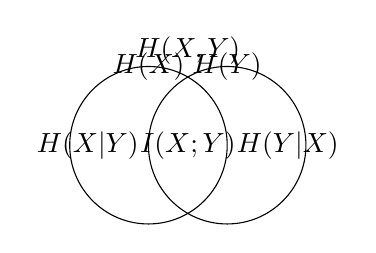
\begin{tikzpicture}
    \node at (0,1) {$H(X)$};
    \node at (1,1) {$H(Y)$};
    \node at (.5,1.2) {$H(X,Y)$};
    \node at (.5,0) {$I(X;Y)$};
    \draw (0,0) circle (1) node [left] {$H(X\vert Y)$};
    \draw (1,0) circle (1) node [right] {$H(Y\vert X)$};
\end{tikzpicture}
\begin{tikzpicture}
    \node at (0,1.4) {所有编码};
    \node at (0,1) {非奇异码};
    \draw (0,.4) circle (.9);
    \node at (0,.6) {唯一可解码};
    \draw (0,.2) circle (.7);
    \draw (0,0) circle (.5) node {瞬时码};
\end{tikzpicture}\\
\begin{tikzpicture}[node distance=10pt]
    \node (input) {正交调幅实现方法1:};
    \node[draw, circle, right=of input] (multiplier 1) {$\times$};
    \node[draw, right=20pt of multiplier 1] (real part) {$2\re$};
    \node[draw, right=15pt of real part] (channel) {信道};
    \node[draw, right=5pt of channel] (Hilbert filter) {希尔伯特滤波器};
    \node[draw, circle, right=20pt of Hilbert filter] (multiplier 2) {$\times$};
    \node[right=of multiplier 2] (output) {};
    \node[above=of multiplier 1] (carrier) {};
    \node[above=of multiplier 2] (carrier removal) {};

    \graph{(input) ->["$u(t)$"] (multiplier 1) ->["$x^+(t)$"] (real part) ->["$x(t)$"] (channel) -> (Hilbert filter) ->["$x^+(t)$"] (multiplier 2) ->["$u(t)$"] (output);
    (carrier) ->["$e^{j2\pi f_ct}$"] (multiplier 1);
    (carrier removal) -> ["$e^{-j2\pi f_ct}$"] (multiplier 2)};
\end{tikzpicture}\\
\begin{tikzpicture}[node distance=10pt]
    \node[draw] (sum of uk'delta) {$\sum_ku_k'\delta(t-kT)$};
    \node[left=50pt of sum of uk'delta] (input 1) {实现方法2:};
    \node[draw, right=5pt of sum of uk'delta] (filter 1) {滤波器$p(t)$};
    \node[draw, circle, right=55pt of filter 1] (multiplier 1) {$\times$};
    \node[above=of multiplier 1] (carrier 1) {};
    \node[draw, circle, below right=2.5pt of multiplier 1] (adder) {$+$};
    \node[right=of adder] (output) {};
    \node[draw, below=of sum of uk'delta] (sum of uk''delta) {$\sum_ku_k''\delta(t-kT)$};
    \node[left=50pt of sum of uk''delta] (input 2) {};
    \node[draw, right=5pt of sum of uk''delta] (filter 2) {滤波器$p(t)$};
    \node[draw, circle, right=55pt of filter 2] (multiplier 2) {$\times$};
    \node[below=of multiplier 2] (carrier 2) {};

    \graph{(input 1) ->["$\{u_k'=\re[u_k]\}$"] (sum of uk'delta) -> (filter 1) ->["$\sum_ku_k'p(t-kT)$"] (multiplier 1) ->[to path={-| (\tikztotarget)}] (adder) ->["$x(t)$"] (output);
    (input 2) ->["$\{u_k''=\im[u_k]\}$"] (sum of uk''delta) -> (filter 2) ->["$\sum_ku_k''p(t-kT)$"] (multiplier 2) ->[to path={-| (\tikztotarget)}] (adder);
    (carrier 1) ->["$\cos 2\pi f_ct$"left] (multiplier 1);
    (carrier 2) ->["$-\sin 2\pi f_ct$"] (multiplier 2)};

    \node[below=30pt of input 2] (input) {$x(t)$};
    \node[draw, circle, above right=2.5pt of input] (multiplier 1) {$\times$};
    \node[draw, right=of multiplier 1] (matched filter 1) {匹配滤波器$q(t)$};
    \node[draw, right=of matched filter 1] (sampler 1) {采样};
    \node[right=20pt of sampler 1] (output 1) {};
    \node[above=of multiplier 1] (carrier removal 1) {};
    \node[draw, circle, below right=2.5pt of input] (multiplier 2) {$\times$};
    \node[draw, right=of multiplier 2] (matched filter 2) {匹配滤波器$q(t)$};
    \node[draw, right=of matched filter 2] (sampler 2) {采样};
    \node[right=20pt of sampler 2] (output 2) {};
    \node[below=of multiplier 2] (carrier removal 2) {};

    \graph{(input) ->[to path={|- (\tikztotarget)}] (multiplier 1) -> (matched filter 1) -> (sampler 1) ->["$\{u_k'\}$"] (output 1);
    (input) ->[to path={|- (\tikztotarget)}] (multiplier 2) -> (matched filter 2) -> (sampler 2) ->["$\{u_k''\}$"] (output 2);
    (carrier removal 1) ->["$\cos 2\pi f_ct$"] (multiplier 1);
    (carrier removal 2) ->["$-\sin 2\pi f_ct$"right] (multiplier 2)};
\end{tikzpicture}
\end{multicols*}
\end{document}